
%---------------------------------------------
%	6. Application & Perform of GNN Algorithm
%---------------------------------------------

%WIt allowed us to generate realistic data emulating a full Silicon LHC detector (see Fig 3), while providing us with the ground truth of particle trajectory membership. Thus, for each event we obtained the... and, as ground truth, the list of points associated to each track. There is a one to one relationship between the true 3D points and the reconstructed ones.

\chapter{Implementation of the GNN Algorithm to the TrackML Model}
\label{chapter-6}

The following chapter focuses on the implementation of the GNN algorithm for the publicly available dataset designed for the Kaggle TrackML challenge \cite{kaggle-trackml}. The TrackML detector emulates a full silicon LHC detector and as such, certain models of the GNN algorithm outlined in Chapter \ref{chapter-5}, are altered for the TrackML detector geometry.

Section \ref{chapter-6-data-prep} describes the structure of the TrackML data and how it was used to build a graph network. Sections \ref{constructing-track-states} and \ref{chapter-6-covariance-derivation} describe the construction of track state estimates. Section \ref{chapter-6-kl-threshold} presents the classifier constructed to determine the optimal KL threshold used within the GMR stage and Section \ref{chapter-6-extrapolation} presents alterations to the extrapolation models used within the Information Aggregation stage. Finally, Section \ref{gnn-kf-implementation} describes specific implementation of KFs. 
 





\section{Data Preparation}
\label{chapter-6-data-prep}

% Make sure the say that the connectiosn between edge pairs are built using the track inclination and a similar predictor method to chapter 4, the edges: spanning up to two layers apart! - REMEMBER edge connections can be 2 layers apart

%Talk specifically about the TrackML data here and how it was prepared. How the trackml hits are converted into nodes and edges. Checks that are put in place in order to make sure there are no hits that have the same module id (more than 2 hits that are simultaneously in the same module and volume and layer).

% the hit-pair predictor used to convert trackml hits and predict compatible edge connections [reference], this methodology was very similar to the chapter 4 hit-pair predictor.

%The main application of the GNN algorithm on the trackML data, the data preparation, what data was exactly used and why, the ML classification algorithm used to build the edge connections. The main results we get from application of this algorithm, the track reconstruction efficiency, the purity metrics, computational performance. Comparison with other algorithms.



\section{Construction of Track State Estimates}
\label{constructing-track-states}

Track parameters in both the transverse $x$-$y$ plane and the $r$-$z$ plane are considered in order to construct track state estimates $X_{ij}$.


\subsection{Parabolic Model}
\label{parabolic-state}

In the $x$-$y$ plane, charged particles experience the influence of the magnetic field, so naturally their trajectories follow a near-parabolic shape. For a given node A, a parabola is formed using the origin O, node A and neighbour node B, illustrated in Figure \ref{fig:gnn-parabolic-model}. The parabola is transformed into the local coordinate system of node A such that the new $x$-axis, $X_A$ goes through the global origin O and node A. The parabolic parameters \{$a, b, c$\} are computed using equations Eq \eqref{eqn:parabolic-equations}. The measurement vector $[m_O \quad m_A \quad m_C]$ is obtained in the coordinate system local to node A, assuming $m_O = 0$ and $m_A = 0$.

\begin{equation}
\begin{aligned}
m_O = ax_{O}^{2} + bx_O + c \\
m_A = c \\
m_B = ax_{B}^{2} + bx_B + c
\end{aligned}
\label{eqn:parabolic-equations}
\end{equation}

\begin{figure}[htbp!] 
    \centering
    \subfloat[]{%
        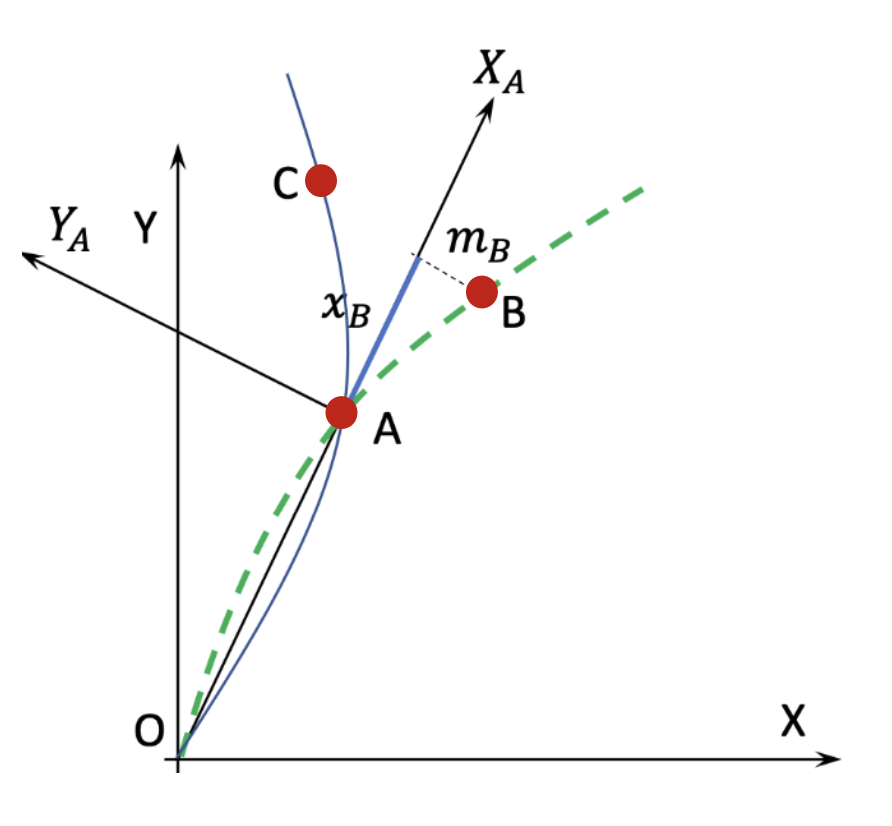
\includegraphics[width=0.43\textwidth]{images/5-gnn-algorithm/parabolic-state-model-1.png}%
        \label{fig:gnn-parabolic-state-1}%
        }%
    \hfill%
    \subfloat[]{%
        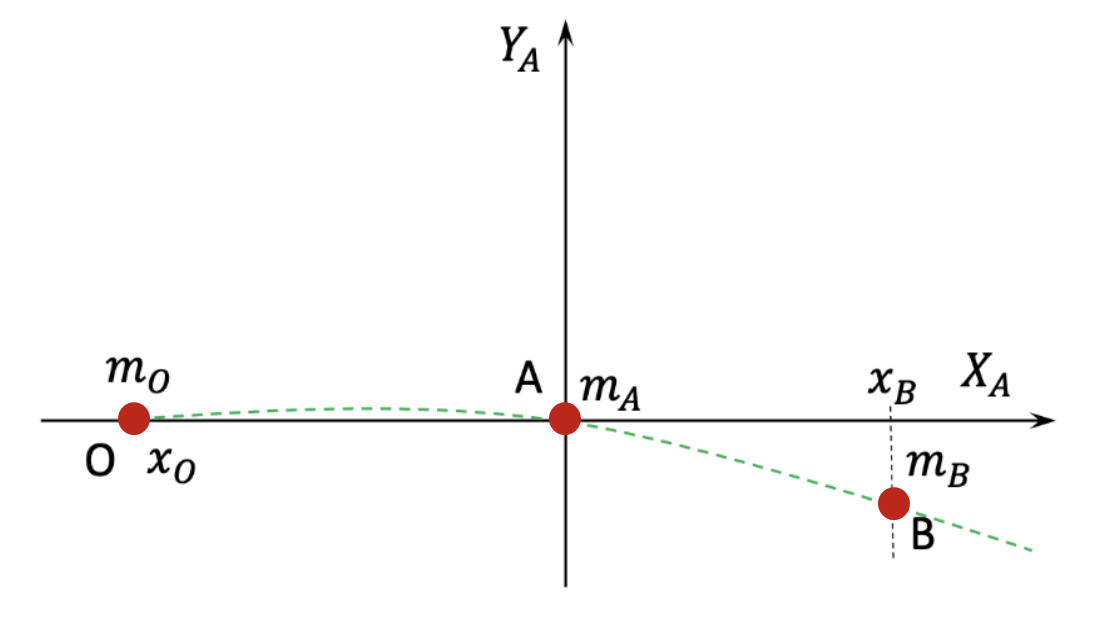
\includegraphics[width=0.57\textwidth]{images/5-gnn-algorithm/parabolic-state-model-2.png}%
        \label{fig:gnn-parabolic-state-2}%
        }%
    \caption{Illustrations of the parabolic model used in the $x$-$y$ plane. a) shows the construction of a parabola between the global origin, O and nodes A - B, as well as a second parabola between O - A - C. b) shows the rotation of the parabola O - A - B into the local coordinate system of node A.}
    \label{fig:gnn-parabolic-model}
\end{figure}


\subsection{Linear Model}
\label{linear-state}

The $r$-$z$ plane is parallel to the direction of travel of the beamline, where tracks follow a linear model. The inverse track inclination between a node and its neighbour, $\tau$, is used and is given by Eq \eqref{eqn:tau-parameter}, where $z_A$, $r_A$ refer to measurements of the node and $z_B$, $r_B$ refer to measurements of its neighbour. $r$ is the square root of the sum in quadrature of the $x$ and $y$ measurements.

\begin{equation}
\tau = \frac{z_A - z_B}{r_A - r_B}
\label{eqn:tau-parameter}
\end{equation}

\subsection{Track State Estimate}

Parabolic parameters $a$ and $b$ in the $x$-$y$ plane, as well as inverse track inclination $\tau$ in the $r$-$z$ plane give an indication of track orientation. For node $i$ and its neighbour $j$, the track state estimate $X_{ij}$ is given by Eq \eqref{eqn:joint-state-vector}

\begin{equation}
X_{ij} = \begin{bmatrix} a \\ b \\ \tau \end{bmatrix}
\label{eqn:joint-state-vector}
\end{equation}






\section{Derivation of Edge State Covariance}
\label{chapter-6-covariance-derivation}

\subsection{Moli\`ere Theory of Multiple Scattering}

The contribution due to multiple scattering is given by Eq \eqref{eqn:moliere-equation}.

\begin{equation}
    \sigma_{ms}^{2} = \frac{13.6 \text{MeV}}{\beta c p} z \sqrt{\frac{x}{X_0}} \left[ 1 + 0.038ln \left( \frac{x}{X_0} \right) \right] 
    \label{eqn:moliere-equation}
\end{equation}

where $p$, $\beta c$, and $z$ are the momentum, velocity, and charge number of the incident particle, and $x/X_0$ is the thickness of the scattering medium, measured in radiation lengths. As the logarithmic correction term is negligible, $\sigma_{ms}^{2}$ becomes

\begin{equation}
    \sigma_{ms}^{2} = \frac{13.6 \text{MeV}}{p} \sqrt{\frac{x}{X_0}}
    \label{eqn:simplified-moliere-equation}
\end{equation}

where $\beta c$, and $z$ are set to 1. The full particle momentum $p$, can be derived using the track curvature $\kappa$ and inverse track inclination $\tau$, where $\kappa$ is a function of parabolic parameters. .... The magnetic field of the TrackML model is such that a particle with transverse momentum $p_\text{T}$ has a radius of trajectory $r = p_\text{T} / 0.3 $. ...what is 0.3 here?

what are x and x0 here? 


\begin{itemize}
\item handling the error/effects due to multiple scattering for the barrel and endcap in slightly different ways
\item how were the edge state covariances dervied and the sigma errors chosen
\end{itemize}
% moliere theory links:
%https://gray.mgh.harvard.edu/attachments/article/337/Techniques%20of%20Proton%20Radiotherapy%20(06)%20Multiple%20Scattering.pdf





\section{The Optimal KL Threshold}
\label{chapter-6-kl-threshold}

To determine the optimal pairwise $d_{KL}$ between track state estimates $X_{ij}$ for a given node, a SVM classifier was trained using pairwise $d_{KL}$ and $\sigma_{e}$ as input features. A MC simulation of $10,000$ particle collision events, each event with ten truth tracks, was used to build a training dataset. Loosely compatible edge connections were formed using a hit-pair predictor based on track inclination angle of neighbouring hits, similar to the graph network constructed in \ref{fig:heat-map}. The feature vector was comprised of $\sigma_{e}$ for a given node and pairwise $d_{KL}$ between its track states. The truth particle was extracted for each pairwise connection, where truth 1 corresponded to hits from both track states originating from the same truth particle, and truth 0 otherwise. 

%The truth data is presented is Figure \ref{fig:KL-distance-truth}.

A SVM was trained to discriminate between the two classes \cite{scikit-learn}, using a polynomial degree three kernel. SVM predictions were adjusted such that the TPR was tuned to 95\% in order to maintain a high purity. The SVM decision boundary was converted into a fast LUT using a similar methodology outlined in Section \ref{LUT-generation} and was directly used within the k-means clustering of the GMR stage. If $d_{KL}$ $\leq$ the predicted threshold for a node with particle $\sigma_e$, then pairwise states were clustered together and merged into a single state $X^M$.

% The predictions and corresponding decision boundary is shown in Figure \ref{fig:KL-distance-predictions}.

Other classification algorithms were explored, however the SVM was the most appropriate to determine a decision boundary to best separate the classes.

% \begin{figure}[htbp!] 
%     \centering
%     \subfloat[Ground truth data from MC simulation]{%
%         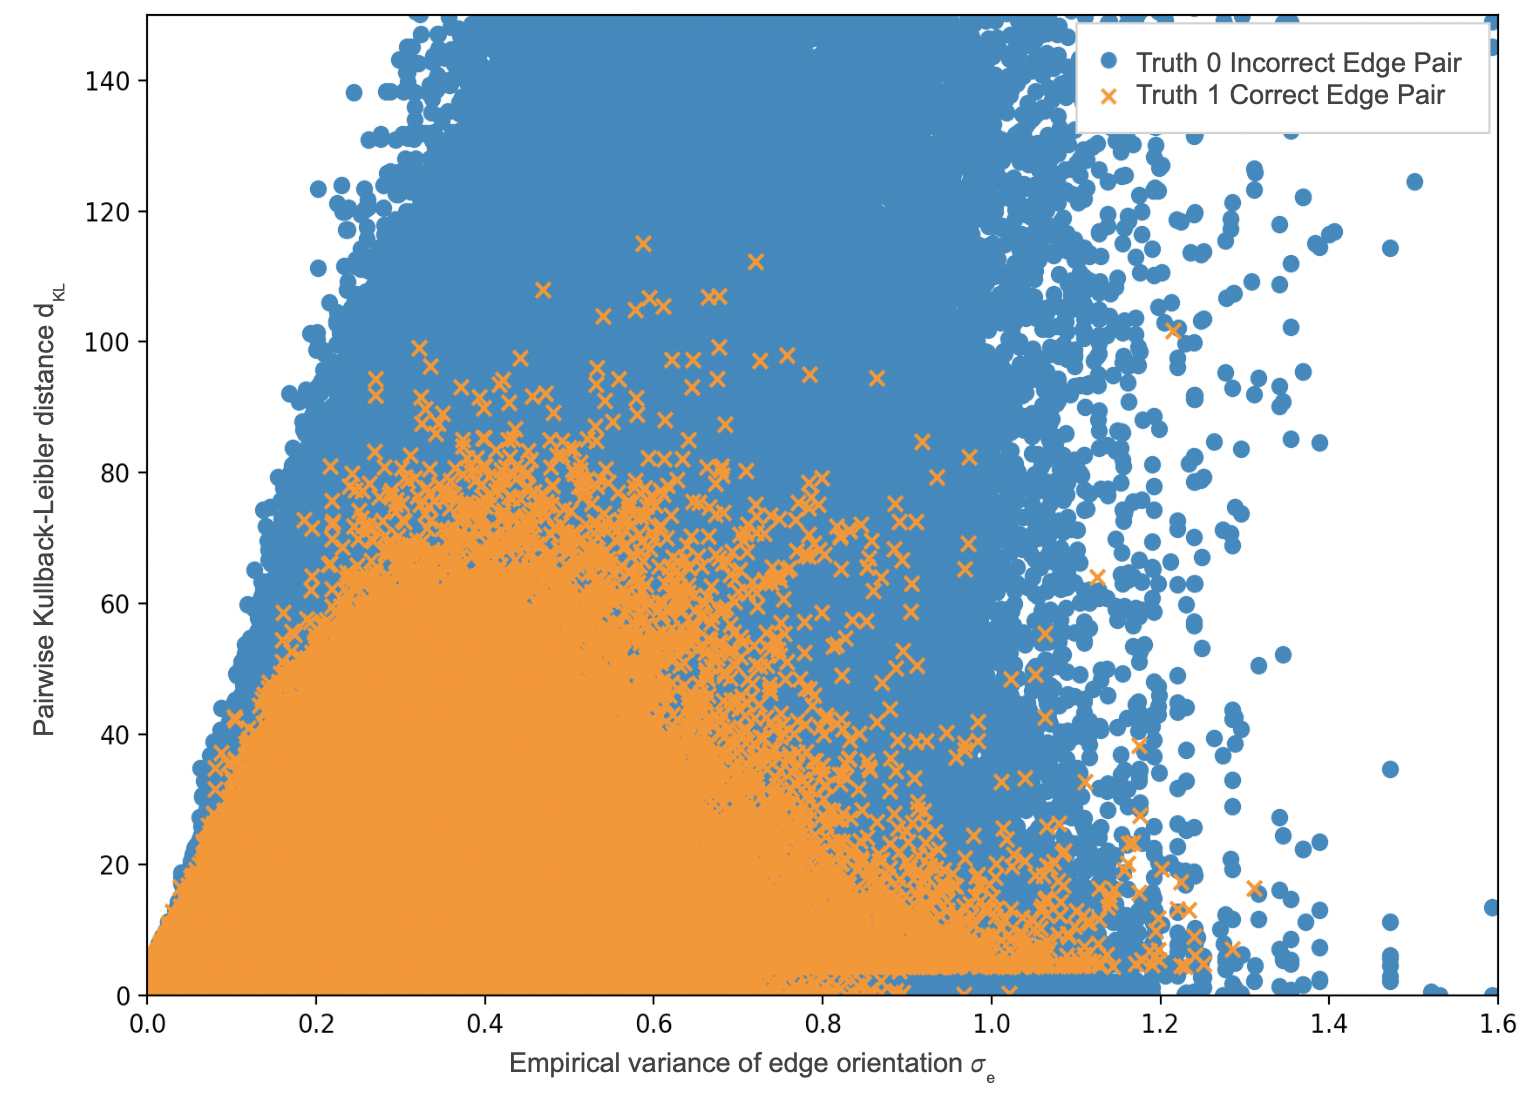
\includegraphics[width=0.85\linewidth]{images/6-results/kl-truth.png}%
%         \label{fig:KL-distance-truth}%
%         }%
%     \hfill%
%     \subfloat[SVM predictions and decision boundary]{%
%         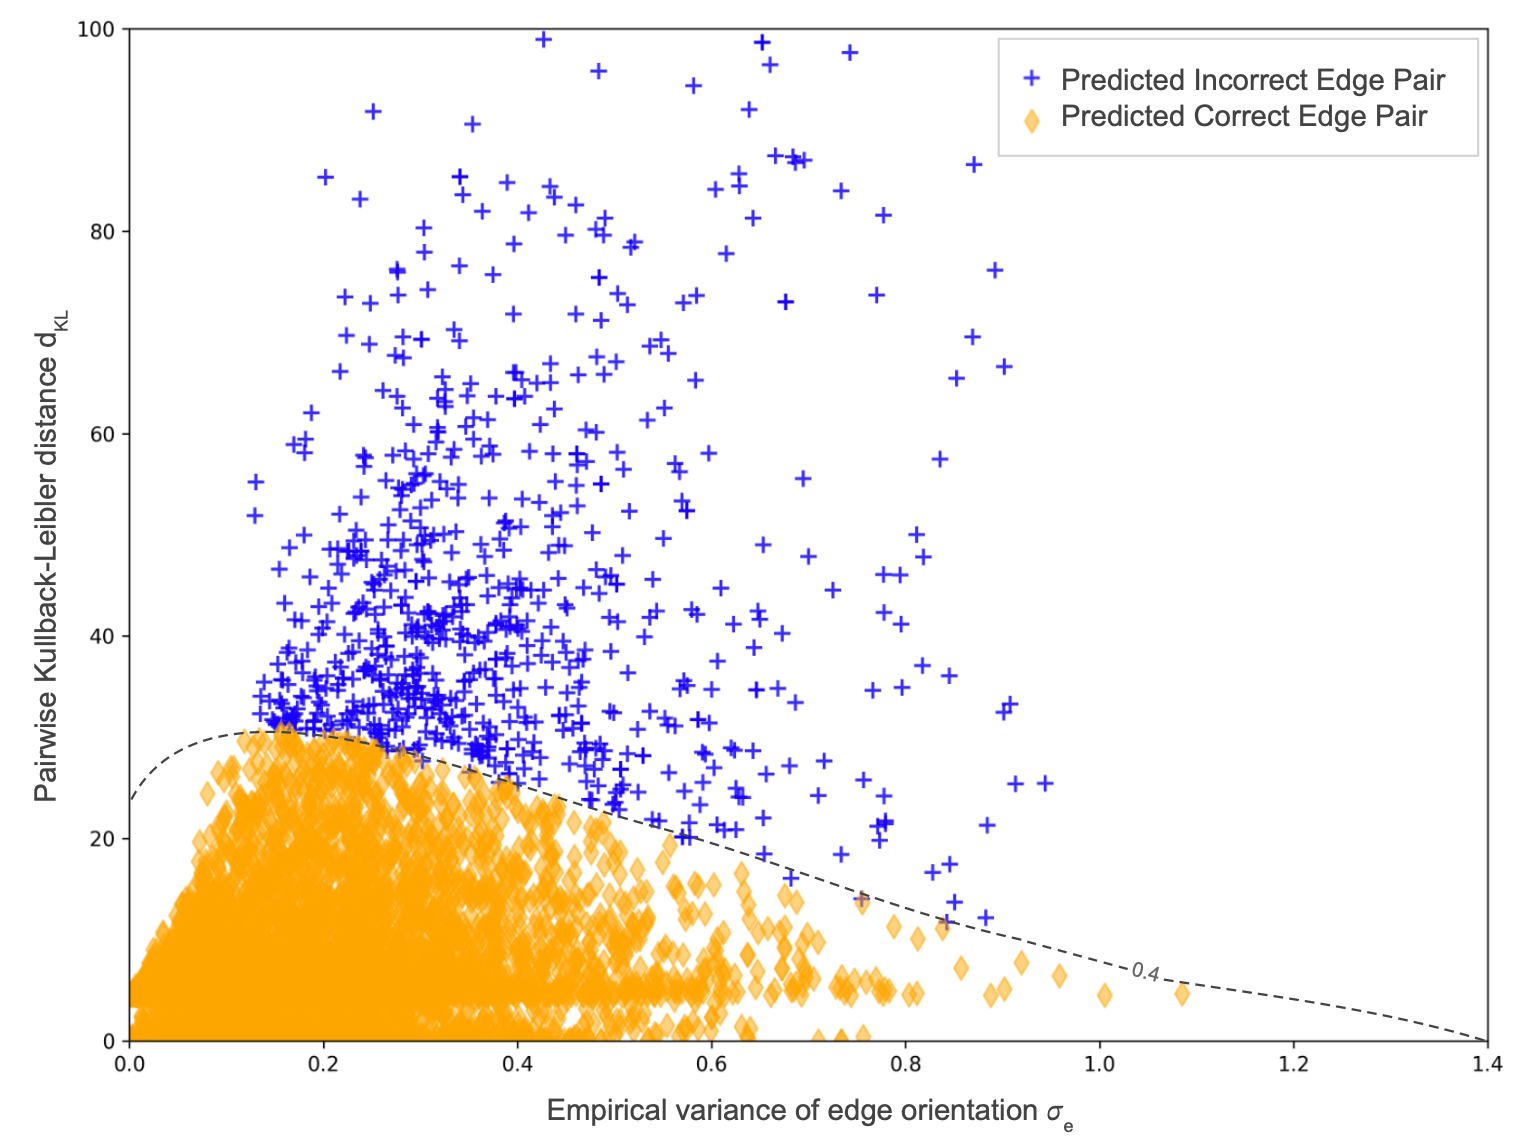
\includegraphics[width=0.85\linewidth]{images/6-results/kl-predictions.png}%
%         \label{fig:KL-distance-predictions}%
%         }%
%     \caption{........}
%     \label{fig:KL-distance}
% \end{figure}





\section{Extrapolation Models}
\label{chapter-6-extrapolation}

\subsection{Parabolic Extrapolation Model}
\begin{itemize}
    \item Information propagation via Message Passing Mechanism
    \item Extrapolation and Validation
    \item Linear and Parabolic model - 2 different extrapolations for xy componenets of state vector and rz componenet, illustrations here
    \item Kalman Filter Update, OU process for correlated noise
\end{itemize}

Mention here that both the linear and parabolic models were used in this instance, where the track state estimate comprised of a 3x1 vector, a, b, tau. The extrapolation and KF update will be different here, different transition Jacobian matrix. Also mention about tuning the chi2 distance thresholds during extrapolation

%The matrix $\widetilde{C}_{ij}$ includes the addition of the process noise $Q$ modelled by the Ornstein-Uhlenbeck (OU) process \cite{OU} which encompasses all material effects. See Section \ref{kf} for further details. The full derivation of $F$ and $Q$ are shown in Appendix \ref{appendix:Appendix-A}

\subsection{Linear Extrapolation Model}


\section{Implementation of Kalman Filters}
\label{gnn-kf-implementation}

\subsection{KF for Extrapolation}
Mention about the OU process noise, for correlated noise etc

\subsection{KF for Track Fitting}

%\begin{itemize}
%\item emphasis on the use of KFs both in information aggregation stage and in track extraction, both are implemented in different ways, is a useful and unique part to this algorithm
%\item OU process noise
%\end{itemize}

